% =============================================================================
% intro.tex
% Rewritten introduction, related work, and real-time environments section.
% Trimmed pass: paragraphs folded, redundant content removed.
%
% Notes:
%   - Uses macros \pigate, \Kset already defined in the main paper.
%   - Cites a few keys that may not yet be in refs.bib:
%       simon1955behavioral, good1971twentyseven, russell1995provably,
%       horvitz1988reasoning. Add or replace as appropriate.
% =============================================================================

% =============================================================================
\section{Introduction}
% =============================================================================

Real-world decision-makers operate under time pressure.
In speed chess, the world does not pause while a player thinks: the clock
runs, the opponent's plan develops, and a brilliant move played a second too
late may be worse than a competent move played on time.
Standard reinforcement learning (RL) sidesteps this entirely.
The Markov Decision Process (MDP) framework that underlies most RL methods
assumes the environment waits for the agent: deliberation is free, and an
agent may take arbitrarily long to choose an action without consequence.

This assumption breaks down in real-time settings, where the world keeps
progressing while the agent decides.
The cost of deliberation in such settings is not wall-clock latency or
abstract compute usage---it is \emph{environmental progression}.
Every additional moment of thinking corresponds to ghosts closing in,
Tetris pieces falling, or a chess clock depleting.
A perfect action that arrives one frame too late is, in a real sense,
not the right action.

\paragraph{The single-budget assumption of existing real-time RL.}
\citet{ramstedt2019rtrl} formalise this concern by fixing the action delay
at exactly one timestep: the agent has one frame to compute its next action,
and the action it emits is applied one frame later.
The resulting Real-Time MDP (RTMDP) is mathematically equivalent to a
1-step constant-delay MDP \citep{walsh2009delayed} and is well-suited to
lightweight reactive policies.
But the framework treats the action delay as a property of the system,
not as a decision the agent makes.
For planners whose computation can usefully span many frames, and for which
the \emph{right} amount of computation is highly state-dependent, fixing
the delay at one leaves the most interesting decision unspecified.

\paragraph{Variable-delay real-time RL.}
We generalise this setting along the axis Ramstedt's framework holds fixed.
In \emph{variable-delay real-time RL}, the agent chooses, at each decision
point, how many timesteps $K$ to spend deliberating before its considered
action is applied to the environment.
This single change introduces three challenges that the fixed-delay
framework does not face.
First, the right delay is state-dependent: some positions reward careful
planning while others demand immediate reaction, and a useful agent must
allocate compute accordingly.
Second, the agent must submit \emph{something} to the environment during
the $K{-}1$ intermediate frames---we call these \emph{filler actions},
which can be either fast reflex actions drawn from the planner's own
policy or no-ops when the environment has an explicit clock.
Third, deciding how long to deliberate is itself a deliberation---if the
meta-decision incurred the same per-frame cost as the planning it controls,
the framework would face the same problem recursively.

\paragraph{Why MCTS, and why simulation count is the right knob.}
We instantiate this setting with AlphaZero-style planners
\citep{silver2018general}, which use Monte Carlo Tree Search (MCTS) at
decision time to refine action selection through repeated simulations
guided by a neural network.
A full description of MCTS is given in Appendix~\ref{app:az_primer}; for
present purposes the key fact is that the number of simulations is a
natural compute knob.
More simulations produce better actions but take longer to run, and we
verify empirically (Figure~\ref{fig:scaling}) that planning quality and
inference latency scale together approximately linearly across our
environments.
This co-scaling is exactly the tradeoff the agent must navigate: better
decisions cost more environmental progression.
It also makes ``how long to plan'' a well-posed, learnable decision
rather than an unbounded budget question.

\paragraph{Meta-reasoning as the framing.}
The problem of choosing $K$ is fundamentally a problem of \emph{meta-reasoning}:
deciding not just what action to take, but how much computation to spend
deciding it.
This connects to a long line of work, beginning with the value-of-computation
framework of \citet{russell1991right}, that asks when a marginal computation
is worth its cost.
Our solution is a lightweight \emph{gating policy}, trained with PPO on
top of a \emph{frozen} AlphaZero planner, that maps each state to a budget
$K \in \Kset$.
The gating policy resolves the recursion problem by construction: a single
gate forward pass takes microseconds, orders of magnitude less than even
one MCTS rollout, so the meta-decision adds negligible real-time cost
even though it is made at every meta-step
(Figure~\ref{fig:realtime-rl-gating-diagram}).
The setting admits two natural physical realisations, distinguished by
where the cost of deliberation manifests in the dynamics:
\emph{committed-action} environments (Pac-Man, real-time Tetris, Snake),
where the world progresses during the $K{-}1$ filler frames, and
\emph{clock} environments (Speed Hex, Speed Go), where a per-player
clock depletes with thinking time.
Section~\ref{sec:envs} formalises both.

\begin{figure}[t]
  \centering
  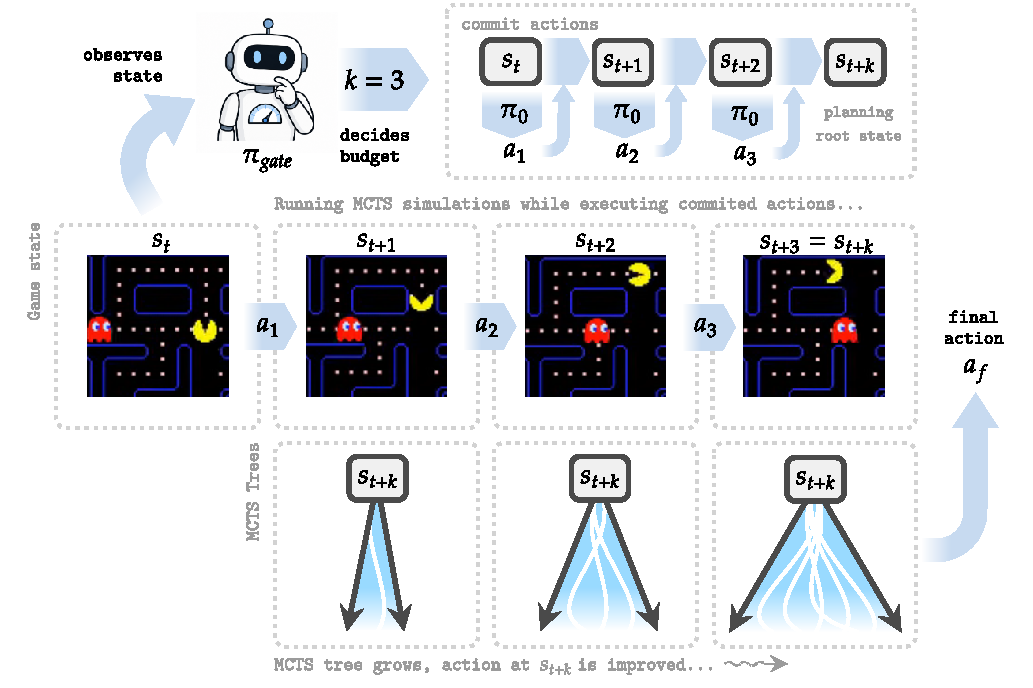
\includegraphics[width=\linewidth]{figures/realtime-rl-gating-diagram.pdf}
  \caption{
    The gating policy chooses, at each meta-step, how long to plan.
    Given the current state, a budget $K \in \Kset$ is selected, which
    determines how many MCTS simulations run and how many filler frames
    elapse before the planner's action lands.
    In committed-action environments the filler frames are reflex actions
    that move the agent through the environment; in clock environments
    they are no-ops that consume the player's clock.
  }
  \label{fig:realtime-rl-gating-diagram}
\end{figure}

\paragraph{Contributions.}
\begin{enumerate}
  \item \textbf{Variable-delay real-time RL.}
    A generalisation of Ramstedt's RTMDP in which the agent chooses how
    many timesteps to deliberate, together with an explicit treatment of
    the two physical realisations---committed-action and clock---that
    naturally arise from this generalisation.
  \item \textbf{Adaptive gating for MCTS budgets.}
    A lightweight gating policy, trained with PPO on top of a frozen
    AlphaZero planner, that selects a per-state planning budget
    $K \in \Kset$.
    The gate's forward pass is cheap enough relative to MCTS that it
    escapes the meta-reasoning recursion problem in practice.
  \item \textbf{Empirical and deployment validation.}
    Across five environments the gating policy outperforms all four
    fixed-budget baselines and standard hand-designed heuristics, and
    the simulation-trained policy transfers to a true two-GPU
    asynchronous deployment with no architectural change.
\end{enumerate}

The learned strategies are interpretable and state-dependent: the gate
plans most deeply when ghosts are nearby in Pac-Man, adopts a strongly
bimodal ``react or plan deeply'' strategy in Tetris that concentrates
$K{=}4$ on dense board states, and raises $K$ in Snake immediately after
the body grows.
In clock environments the same trained policy redistributes mass toward
deeper search when more clock remains.
In two-GPU deployment across three environments, three GPU classes, and
five frame rates, returns transfer cleanly and gate inference adds
negligible overhead relative to MCTS latency, closing the loop on the
recursion concern empirically.


% =============================================================================
\section{Background and Related Work}
% =============================================================================

\paragraph{Real-time RL and delayed MDPs.}
The standard MDP assumes the environment waits during action selection.
\citet{travnik2018reactive} flagged this as a fundamental mismatch with
real-time interaction, and \citet{ramstedt2019rtrl} formalised an alternative
in which the agent has exactly one timestep to compute its next action,
mathematically equivalent to a 1-step constant-delay
MDP~\citep{walsh2009delayed}.
Subsequent work extends this to fixed action and observation delays of
larger length~\citep{derman2021delayed,bouteiller2021random,katsikopoulos2003markov},
to concurrent control~\citep{xiao2020thinking}, and to asynchronous and
pipelined architectures that mitigate inference cost~\citep{riemer2025staggered,
anokhin2025handling}.
Across this body of work the action delay is a property of the system
imposed on the agent.
We instead let the agent \emph{choose} its delay $K$ at each decision
point, generalising RTMDP from a fixed 1-step delay to a variable-delay
setting in which the choice itself is the central learning problem; we
formalise the resulting SMDP in Section~\ref{sec:envs} and
Appendix~\ref{app:rtrl_smdp}.

\paragraph{Value of computation and meta-reasoning.}
The view that rational agents must reason not only about what to do but
about how much to think traces back to bounded
rationality~\citep{simon1955behavioral} and Good's \emph{Type II
rationality}~\citep{good1971twentyseven}.
\citet{russell1991right} made this operational by defining the
\emph{value of computation} (VOC) as the expected improvement in decision
quality minus its cost, and \citet{russell1995provably}'s
bounded-optimality framework reframed rational agency as the optimal use
of fixed computational resources.
Anytime algorithms~\citep{dean1988analysis,zilberstein1996using,
likhachev2003ara,korf1990rta} produce monotonically improving answers as
more time is given, and Bayesian flexible-computation
methods~\citep{horvitz1988reasoning} formalise when to stop.
Applied to MCTS, value-of-computation ideas yield Bayesian formulations
of which simulation to run next~\citep{hay2012selecting,tolpin2012simple,
sezener2020static,lin2015metareasoning}, while classical chess- and
Go-engine time management~\citep{baier2016time,huang2010timemanagement,
baudis2012pachi} allocates clock per move via hand-designed heuristics.
The cognitive-science literature models bounded deliberation itself as a
meta-MDP whose actions are computations~\citep{lieder2017strategy,
griffiths2019doing,callaway2018learning,cope_learning_2023} and shows
empirically that humans allocate planning effort to high-stakes
decisions in ways predicted by this model.
Our gating policy is, in this lineage, a learned VOC estimator---a
deep-RL instantiation of the meta-MDP idea---that operates macroscopically
on total budget per decision rather than microscopically on which
simulation to run next.

\paragraph{Adaptive compute in model-based RL.}
The closest neighbours to our work \emph{learn} to allocate planning
compute on top of a model-based RL agent.
Metacontrol~\citep{hamrick2017metacontrol} chooses how many imagination
steps to run; Thinker and Dynamic Thinker~\citep{chung2023thinker,
wang2024dynamic} let the agent itself decide when to imagine alternative
trajectories on top of a learned world model; Adaptive
Lookahead~\citep{dalal2022adaptive} learns a state-dependent tree-search
horizon.
\citet{hamrick2021role} provides the strongest empirical motivation:
shallow MuZero trees often suffice, and the marginal value of additional
simulations varies sharply by state.
AlphaZero-family planners themselves~\citep{silver2018general,
schrittwieser2020muzero,danihelka2022policy} treat MCTS budget as a
fixed deployment hyperparameter.
Our setting differs from all of these in that the cost of additional
planning is paid in environmental progression rather than in artificial
reward shaping, and our gate operates over a frozen planner with no
joint training.
Other axes of ``learning to search''~\citep{guez2018mctsnets,
farquhar2018treeqn,hamrick2020save,racaniere2017i2a} modify a planner's
internal behaviour rather than its budget; we hold the planner fixed and
control only how long it runs.

\paragraph{Adaptive compute in language models.}
The same idea has been independently developed for sequence models.
PonderNet and adaptive computation time~\citep{graves2016act,
banino2021pondernet,schuster2022calm} learn per-input halting; test-time
compute scaling~\citep{snell2024scaling,deepseek2025r1,muennighoff2025s1}
and RL-trained reasoning-length controllers~\citep{aggarwal2025l1,
muppidi2025predictive,fang2025thinkless,shen2025dast} learn per-query
thinking budgets; cascaded routing~\citep{kim2023bigl,chen2023frugalgpt,
ong2025routellm} defers easy queries to cheap models.
The shared thesis is that a small learned policy can profitably decide
how much computation to spend per decision.
Our setting differs structurally: the cost is endogenous to the
environment dynamics, so thinking longer changes the world the agent
eventually acts in, rather than incurring an external penalty.


% =============================================================================
\section{Variable-Delay Real-Time RL}
\label{sec:envs}
% =============================================================================

This section formalises the variable-delay setting and describes the
two physical realisations we study.
We treat the formalism first because the two environment families
(committed-action and clock) are best understood as two ways of
instantiating the same underlying generalisation of RTMDP.

\subsection{From fixed to variable action delay}

\citet{ramstedt2019rtrl}'s RTMDP fixes the action delay at exactly one
timestep.
The augmented state $\mathbf{x}_t = (s_t, a_t)$ carries the action
selected at $t{-}1$, and the transition kernel is
\begin{equation}
  p(\mathbf{x}_{t+1} \mid \mathbf{x}_t, \hat{a}_t)
  = p(s_{t+1} \mid s_t, a_t)\,\delta(a_{t+1} - \hat{a}_t),
\end{equation}
which passes the newly emitted action $\hat{a}_t$ forward to land at
frame $t{+}1$.
This framework is well-suited to lightweight policies whose evaluation
fits within one frame, but the delay is a property of the system rather
than a quantity the agent reasons about.

We extend RTMDP along two axes.
First, we allow the action delay to vary per decision: at each meta-step
the agent's gating policy $\pigate$ chooses a budget $K_t \in \Kset$,
and the agent's considered action lands $K_t$ frames later.
Second, because the environment continues to evolve over those $K_t$
frames, we must specify what is submitted to the environment during the
$K_t{-}1$ intermediate frames---the filler actions introduced above.
The choice of filler distinguishes the two physical realisations: in
committed-action environments the filler is a reflex action that moves
the agent in the world, and in clock environments the filler is a no-op
that simply consumes the player's clock.

A useful framing is that each meta-decision selects an
\emph{option}~\citep{sutton1999between,bacon2017optioncritic} of length
$K_t$: $K_t{-}1$ filler steps drawn from a fixed reflex distribution,
followed by one action selected by MCTS.
The induced process is a discrete-time semi-Markov decision process
(SMDP) whose holding times are chosen by the meta-policy, with
meta-reward
\begin{equation}
  R_t \;=\; \sum_{k=0}^{K_t - 1} \gamma^k \, r_{t+k}
\end{equation}
and per-meta-step discount $\gamma^{K_t}$, exactly as in the standard
options formulation.
The Bellman equation for the meta-value is
\begin{equation}
  V(s_t)
  \;=\;
  \mathbb{E}_{K_t \sim \pigate}\!\left[
    R_t + \gamma^{K_t}\, V(s_{t + K_t})
  \right],
  \label{eq:smdp}
\end{equation}
and we adapt Generalized Advantage Estimation~\citep{schulman2015high}
to carry the per-step discount $\gamma^{K_t}$ through the advantage
computation.
In simulation this is a discrete SMDP with deterministic holding time
set by the chosen $K_t$; in real deployment, MCTS execution time is
slightly stochastic, so the hardware system is closer to a genuine
continuous-time SMDP.
Appendix~\ref{app:rtrl_smdp} works through the formal distinction.

A central design principle across both realisations is that the
planning process is \emph{cost-aware by construction}: nothing about the
cost of thinking is added via reward shaping.
Either the MCTS tree explicitly simulates how the world evolves during
the planning delay, or the network is trained on observations that
include the remaining time budget.
We now describe both realisations and the mechanism by which each is
cost-aware.

\subsection{Committed-action environments: Pac-Man, real-time Tetris, Snake}

In committed-action environments, acting and planning happen
concurrently, and cost-awareness is built directly into the MCTS
search.
When the gating policy selects $K$, it reserves $K$ environment frames
for the planner.
The agent emits $K{-}1$ filler actions---reflex argmax actions drawn
from the planner's own policy network, computed via a single forward
pass in roughly two milliseconds---while the full MCTS runs in the
background.
On the $K$-th frame the planner's chosen action is applied.
The MCTS tree's recurrent function rolls out the same $K{-}1$-step
reflex trajectory that the agent will actually execute, so the search
is conducted over the future the planner will land in, not over a
fictitious paused world.
The cost of deeper planning is therefore exactly $K{-}1$ additional
frames of world progression before the carefully chosen action lands.

We instantiate this realisation in three environments derived from
Jumanji~\citep{bonnet2024jumanji}: Pac-Man, Snake, and a real-time
variant of Tetris.
The source of progression differs across environments---ghost motion in
Pac-Man, gravity in real-time Tetris, body elongation in Snake---but
the structural property is shared: a deeper plan arrives later, after
the world has already changed.
We modify Jumanji Tetris so that gravity advances the piece in real
time; environment-specific details are in Appendix~\ref{app:envs_tetris}.

\paragraph{Equal compute per frame.}
All budget options in $\Kset$ are calibrated to carry the same number
of MCTS simulations per game frame: at budget $K$ the planner runs
$K \times 32$ simulations over $K$ environment frames, so each frame
receives 32 simulations on average regardless of $K$
(Table~\ref{tab:budget}).
Differences in performance therefore reflect \emph{when} compute is
allocated, not how much total compute is consumed.

\begin{table}[h]
  \centering
  \caption{Committed-action environments: all budget options share 32
    MCTS simulations per game frame.}
  \label{tab:budget}
  \small
  \begin{tabular}{lcccc}
    \toprule
    & $K{=}1$ & $K{=}2$ & $K{=}3$ & $K{=}4$ \\
    \midrule
    MCTS simulations       & 32 & 64 & 96 & 128 \\
    Filler actions         & 0  & 1  & 2  & 3   \\
    Simulations per frame  & 32 & 32 & 32 & 32  \\
    \bottomrule
  \end{tabular}
\end{table}

\subsection{Clock environments: Speed Hex and Speed Go}

In clock environments the board does not evolve while a player
deliberates, but each player has an explicit clock that depletes with
thinking time.
Filler actions are no-ops, only the planner's chosen action takes
effect on the board, and the corresponding time cost is deducted from
the clock after the move is played.
Cost-awareness here is built into the value network rather than the
search tree: the remaining clock for both players is part of the
observation, and the network is trained on clock-augmented states
throughout self-play, so its value estimates already price in the cost
of thinking.
A position evaluated with little time remaining is worth less than the
same position with ample time, even though the board itself is
identical.
MCTS therefore operates on board-only dynamics during simulation
without losing cost-awareness, because the cost is baked into the
priors and values it consumes.
We instantiate this realisation in Speed Hex (11$\times$11) and Speed
Go (9$\times$9), both built on \texttt{pgx}; in both cases the central
decision is not only \emph{which} move to play but \emph{how much} of
the remaining clock to spend before playing it.

\paragraph{Simulation-option calibration.}
For clock environments the equal-compute-per-frame constraint does not
apply, so we calibrate the simulation options $\Kset$ separately to
ensure each option represents a meaningfully distinct tradeoff between
inference latency and planning quality.
Calibration details and the resulting option sets---$\{2,8,32,128\}$
simulations for Speed Hex and $\{16,32,64,96\}$ for Speed Go---are in
Appendix~\ref{app:sim_calibration}.